% ============================================================================
%  SCS 4203 - Assignment 2
%  Technical report for the SL Tourism Multimodal RAG system
%
%  Compiles with pdfLaTeX. No external files are needed.
%  Before submitting, fill in the two index numbers on the title page and
%  check the Acknowledgements section.
% ============================================================================

\documentclass[11pt,a4paper]{article}

\usepackage[T1]{fontenc}
\usepackage[utf8]{inputenc}
\usepackage[margin=2.5cm]{geometry}
\usepackage{graphicx}
\usepackage{booktabs}
\usepackage{longtable}
\usepackage{amsmath}
\usepackage{amssymb}   % \checkmark
\usepackage{xcolor}
\usepackage{listings}
\usepackage{caption}
\usepackage{enumitem}
\usepackage{tikz}
\usetikzlibrary{arrows.meta,positioning,fit,backgrounds}
\usepackage[hidelinks]{hyperref}

% ---------------------------------------------------------------- listings --
\definecolor{codebg}{RGB}{247,245,241}
\definecolor{codekw}{RGB}{14,92,91}
\definecolor{codecm}{RGB}{110,120,118}
\definecolor{codestr}{RGB}{160,70,45}

\lstdefinestyle{plain}{
  backgroundcolor=\color{codebg},
  basicstyle=\ttfamily\footnotesize,
  keywordstyle=\color{codekw}\bfseries,
  commentstyle=\color{codecm}\itshape,
  stringstyle=\color{codestr},
  breaklines=true,
  breakatwhitespace=true,
  showstringspaces=false,
  frame=single,
  rulecolor=\color{gray!30},
  framesep=5pt,
  xleftmargin=6pt,
  captionpos=b,
  tabsize=2,
}
\lstset{style=plain}

\lstdefinelanguage{sqlx}{
  morekeywords={CREATE,TABLE,VIEW,INDEX,SELECT,FROM,WHERE,LEFT,JOIN,ON,PRIMARY,
    KEY,REFERENCES,ON,DELETE,CASCADE,NOT,NULL,CHECK,IN,ALTER,ADD,COLUMN,
    GENERATED,ALWAYS,AS,STORED,USING,GIN,ORDER,BY,LIMIT,AND,OR,SERIAL,TEXT,
    REAL,BOOLEAN,TIMESTAMP,DEFAULT,CURRENT_TIMESTAMP,ANY,DISTINCT,GROUP},
  sensitive=false,
  morecomment=[l]{--},
  morestring=[b]',
}

\captionsetup{font=small,labelfont=bf}

\title{\vspace{-1.5cm}\textbf{A Multimodal Retrieval-Augmented Generation System\\
for Sri Lankan Tourist Attractions}}

\author{%
  Murshid \quad\textbar\quad Index No: \rule{2.5cm}{0.4pt}\\[2pt]
  Simaak \quad\textbar\quad Index No: \rule{2.5cm}{0.4pt}\\[6pt]
  \normalsize SCS 4203 --- Assignment 2
}
\date{August 2026}

\begin{document}
\maketitle

\begin{abstract}
\noindent
This report describes a multimodal retrieval-augmented generation (RAG) system
built over a knowledge base of 40 Sri Lankan tourist attractions spanning four
categories: beaches, mountains, national parks and historical sites. Structured
attributes are held in PostgreSQL using a normalised supertype/subtype schema;
descriptive text and photographs are embedded into ChromaDB using
\texttt{all-MiniLM-L6-v2} and CLIP ViT-B/32 respectively. The system supports
four query modes --- structured, semantic, image and hybrid --- exposed through
a FastAPI backend. Hybrid queries are classified by a Gemini structured-output
router, dispatched to several retrievers in parallel and merged with Reciprocal
Rank Fusion. We report measurements showing that lexical and dense retrieval
fail on disjoint query types, that fusing them recovers both, and that the
LLM router classifies our test queries correctly where a keyword heuristic does
not. We also document a defect found during development in which structured SQL
results, fused as if they were a ranked list, degraded hybrid retrieval below
the quality of a single retriever.
\end{abstract}

\tableofcontents
\newpage

% ===========================================================================
\section{Introduction}
% ===========================================================================

A conventional tourism search interface forces the user to know in advance which
attribute they want to filter on. A visitor who asks ``where can I see leopards
on a safari?'' is not filtering on a column; they are describing an experience.
A visitor who asks ``which UNESCO sites in Matale are worth a day trip?'' is
doing both at once --- naming a concrete filter and a subjective quality in the
same sentence.

This system addresses that by combining three retrieval strategies over one
knowledge base and letting a language model decide which to apply. It supports:

\begin{itemize}[itemsep=2pt]
  \item \textbf{Structured queries} --- factual lookups answered by SQL filters
        over the relational database.
  \item \textbf{Semantic queries} --- meaning-based matching against written
        descriptions using sentence embeddings.
  \item \textbf{Image retrieval queries} --- visual similarity search using CLIP
        embeddings, driven either by an uploaded photograph or by a textual
        description of appearance.
  \item \textbf{Hybrid queries} --- a combination of the above, merged into a
        single ranking and used to ground a generated natural-language answer.
\end{itemize}

\subsection{Knowledge base scope}

Four categories were selected from those permitted by the brief, on the basis
that sufficient structured data, descriptive text and openly licensed imagery
were available for each. Table~\ref{tab:kb} summarises the contents.

\begin{table}[h]
\centering
\small
\begin{tabular}{lccc}
\toprule
\textbf{Category} & \textbf{Attractions} & \textbf{With imagery} & \textbf{Descriptions} \\
\midrule
Beaches           & 10 & 8 & 10 \\
Mountains         & 10 & 7 & 10 \\
National parks    & 10 & 6 & 10 \\
Historical sites  & 10 & 3 & 10 \\
\midrule
\textbf{Total}    & \textbf{40} & \textbf{24} & \textbf{40} \\
\bottomrule
\end{tabular}
\caption{Knowledge base composition. Every attraction has structured attributes
and a written description; image coverage is uneven for reasons discussed in
Section~\ref{sec:limitations}.}
\label{tab:kb}
\end{table}

% ===========================================================================
\section{System Architecture}
% ===========================================================================

The system is divided into four layers with an enforced boundary between the
interface and everything below it (Figure~\ref{fig:arch}).

\begin{figure}[h]
\centering
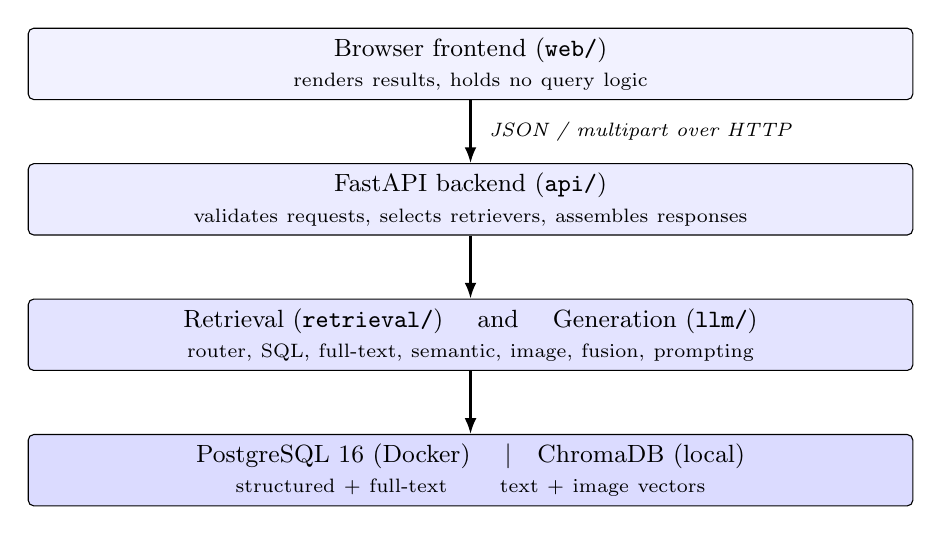
\begin{tikzpicture}[
    node distance=8mm,
    box/.style={draw,rounded corners=2pt,align=center,minimum height=9mm,
                text width=11cm,font=\small},
    lbl/.style={font=\scriptsize\itshape,align=center},
    arr/.style={-{Latex[length=2mm]},thick}
  ]
  \node[box,fill=blue!5] (ui) {Browser frontend (\texttt{web/})\\
        \scriptsize renders results, holds no query logic};
  \node[box,fill=blue!8,below=of ui] (api) {FastAPI backend (\texttt{api/})\\
        \scriptsize validates requests, selects retrievers, assembles responses};
  \node[box,fill=blue!11,below=of api] (log) {Retrieval (\texttt{retrieval/})
        \quad and \quad Generation (\texttt{llm/})\\
        \scriptsize router, SQL, full-text, semantic, image, fusion, prompting};
  \node[box,fill=blue!14,below=of log] (st) {PostgreSQL 16 (Docker)
        \quad\textbar\quad ChromaDB (local)\\
        \scriptsize structured + full-text \qquad text + image vectors};

  \draw[arr] (ui) -- node[right,lbl]{~JSON / multipart over HTTP} (api);
  \draw[arr] (api) -- (log);
  \draw[arr] (log) -- (st);
\end{tikzpicture}
\caption{Layered architecture. The frontend reaches the data only through the
HTTP API.}
\label{fig:arch}
\end{figure}

\subsection{Why the interface goes through an API}

The frontend is served by the API itself, so it could have imported the
retrieval modules directly and avoided a network hop. It does not, for three
reasons.

\begin{enumerate}[itemsep=2pt]
  \item \textbf{The retrieval pipeline remains independently demonstrable.}
        FastAPI generates OpenAPI documentation at \texttt{/docs}, so every
        query type can be exercised and inspected without any interface at all.
  \item \textbf{Query logic cannot migrate into the interface.} With a process
        boundary in between there is no opportunity to add a shortcut that
        bypasses the retrieval layer.
  \item \textbf{Parallel development.} The two halves were built against a fixed
        contract (\texttt{api/schemas.py}) rather than against each other's
        internals.
\end{enumerate}

The cost is one HTTP round trip per query, which is negligible beside embedding
and language-model latency.

\subsection{Module responsibilities}

\begin{table}[h]
\centering
\small
\begin{tabular}{lp{10.2cm}}
\toprule
\textbf{Package} & \textbf{Responsibility} \\
\midrule
\texttt{db/}         & Schema definition, connection pooling, CSV ingestion. The only package that opens database connections. \\
\texttt{embeddings/} & Encoding text and images into ChromaDB collections. \\
\texttt{retrieval/}  & The five retrievers plus fusion and routing. Returns plain dictionaries, never ORM objects, so results from different retrievers can be merged without type conversion. \\
\texttt{llm/}        & Prompt context assembly and answer generation. Receives already-retrieved rows and never queries storage itself. \\
\texttt{api/}        & Request validation, retriever selection, response assembly. \\
\texttt{web/}        & Presentation only. Opens no files and no database connections. \\
\bottomrule
\end{tabular}
\caption{Package responsibilities.}
\end{table}

% ===========================================================================
\section{Database Design}
% ===========================================================================

\subsection{The modelling problem}

The four categories share some attributes and differ in others. A beach has a
water quality and a surf break; a mountain has a height and a trekking
difficulty; a national park has a habitat and a conservation status.

The naive approach --- a single wide \texttt{attractions} table carrying every
column --- produces a \emph{sparse table}. A beach row would carry eleven
permanently \texttt{NULL} columns, and those nulls would be structural rather
than unknown, so a predicate such as \texttt{height\_m IS NULL} could not
distinguish ``this is not a mountain'' from ``we have not measured it''. Adding
a fifth category would widen every existing row.

\subsection{Class-table inheritance}

We instead use the supertype/subtype pattern: one core table holding the shared
attributes, plus one detail table per category holding only that category's
attributes, joined one-to-one.

\begin{lstlisting}[language=sqlx,caption={Core table and one representative
detail table.}]
CREATE TABLE attractions (
    id            TEXT PRIMARY KEY,
    name          TEXT NOT NULL,
    category      TEXT NOT NULL CHECK (category IN
                    ('beach','mountain','national_park','historical_site')),
    location      TEXT,
    district      TEXT,
    latitude      REAL,
    longitude     REAL,
    entrance_fee  TEXT,
    accessibility TEXT CHECK (accessibility IN ('easy','moderate','difficult')),
    best_season   TEXT,
    created_at    TIMESTAMP DEFAULT CURRENT_TIMESTAMP
);

CREATE TABLE mountain_details (
    attraction_id       TEXT PRIMARY KEY REFERENCES attractions(id)
                                          ON DELETE CASCADE,
    height_m            REAL,
    trekking_difficulty TEXT,
    duration_hours      REAL
);
\end{lstlisting}

In each detail table the primary key \emph{is} the foreign key. That single
declaration does three jobs: it enforces the one-to-one cardinality, since a
primary key cannot repeat; it guarantees referential integrity; and
\texttt{ON DELETE CASCADE} removes the detail row automatically when the
attraction is deleted.

Images are a separate one-to-many table, since an attraction may have several
photographs.

\paragraph{Benefits.} No structural nulls; category-specific constraints become
possible (\texttt{height\_m} could be made \texttt{NOT NULL} for mountains
without affecting beaches); and a fifth category is a new table rather than a
migration of existing rows.

\paragraph{Cost.} Every read requires joins. This is what the view addresses.

\subsection{The flattening view}

\begin{lstlisting}[language=sqlx,caption={\texttt{attractions\_full} reassembles
the subtypes so application code never writes the joins.}]
CREATE VIEW attractions_full AS
SELECT a.*,
       b.activity_type, b.water_quality, b.surf_break,
       m.height_m, m.trekking_difficulty, m.duration_hours,
       np.conservation_status, np.habitat, np.area_sq_km, np.notable_wildlife,
       h.historical_period, h.architectural_style, h.unesco_status
FROM attractions a
LEFT JOIN beach_details b            ON a.id = b.attraction_id
LEFT JOIN mountain_details m         ON a.id = m.attraction_id
LEFT JOIN national_park_details np   ON a.id = np.attraction_id
LEFT JOIN historical_site_details h  ON a.id = h.attraction_id;
\end{lstlisting}

Application code selects from this view exclusively. The normalisation benefit
is retained at the storage layer while queries stay as simple as they would be
against a wide table.

The view does reintroduce nulls in its \emph{output} --- a beach row has a null
\texttt{height\_m}. These are stripped in
\texttt{retrieval/sql\_query.py:clean\_row()} using a per-category allowlist
before results leave the retrieval layer. The distinction matters: the nulls are
a presentation artefact of the view, not stored data.

\subsection{Full-text search}

\begin{lstlisting}[language=sqlx,caption={Generated tsvector column with a GIN
index.}]
ALTER TABLE attractions ADD COLUMN search_vector tsvector
    GENERATED ALWAYS AS (
        to_tsvector('english',
            name || ' ' || coalesce(location,'') || ' ' || coalesce(district,''))
    ) STORED;

CREATE INDEX idx_attractions_search ON attractions USING GIN (search_vector);
\end{lstlisting}

A \emph{generated column} was chosen over a trigger: PostgreSQL keeps it
synchronised on every insert and update with no maintenance code and no
possibility of the two drifting apart. The \texttt{coalesce} calls are required
because a null would propagate through the concatenation and blank the entire
vector for any attraction missing a location.

\subsection{Indexes and constraints}

\begin{table}[h]
\centering
\small
\begin{tabular}{lll}
\toprule
\textbf{Index} & \textbf{Column} & \textbf{Rationale} \\
\midrule
\texttt{idx\_attractions\_category} & \texttt{category} & Filtered on in nearly every structured query \\
\texttt{idx\_attractions\_district} & \texttt{district} & Second most common filter \\
\texttt{idx\_images\_attraction}    & \texttt{images.attraction\_id} & Batched image lookup per result set \\
\texttt{idx\_attractions\_search}   & \texttt{search\_vector} (GIN) & Full-text matching \\
\bottomrule
\end{tabular}
\caption{Declared indexes.}
\end{table}

At 40 rows these indexes are not load-bearing --- PostgreSQL will sequentially
scan a table this small regardless. They are declared because they express the
intended access pattern and would become significant at realistic scale.

\texttt{CHECK} constraints are used in preference to application-level
validation so that a malformed CSV row fails at import time rather than
surfacing later as a silently broken filter.

\subsection{Ingestion}

The source CSVs are deliberately flat --- one row per attraction --- because
they are maintained by hand in a spreadsheet. \texttt{db/init\_db.py} performs
the decomposition:

\begin{center}
\small
\texttt{beaches.csv row} $\longrightarrow$
\texttt{attractions} (shared columns, \texttt{category='beach'}) $+$
\texttt{beach\_details} (category columns)
\end{center}

The per-category configuration lives in a single dictionary at the top of the
loader, recording each file's category value, detail table, columns, and which
columns require boolean or numeric coercion. Adding a category requires one
entry there and one table in \texttt{schema.sql}.

Images are registered separately by matching filenames against attraction
identifiers, so \texttt{sigiriya.jpg} and \texttt{sigiriya\_2.jpg} both belong
to \texttt{sigiriya}. The match selects the \emph{longest} candidate identifier,
so that \texttt{little\_adams\_peak.jpg} is not incorrectly claimed by
\texttt{adams\_peak}.

% ===========================================================================
\section{Embedding Generation}
% ===========================================================================

Two independent vector spaces are maintained in ChromaDB with local persistence.

\begin{table}[h]
\centering
\small
\begin{tabular}{llcl}
\toprule
\textbf{Collection} & \textbf{Model} & \textbf{Dim.} & \textbf{Unit embedded} \\
\midrule
\texttt{text\_descriptions} & \texttt{all-MiniLM-L6-v2} & 384 & one document per attraction \\
\texttt{image\_embeddings}  & \texttt{openai/clip-vit-base-patch32} & 512 & one vector per image file \\
\bottomrule
\end{tabular}
\caption{Embedding collections.}
\end{table}

The two spaces are never compared against one another. A MiniLM vector and a
CLIP vector may describe the same attraction but occupy unrelated coordinate
systems; a distance between them would be meaningless. They are combined only at
the level of \emph{rank}, through fusion.

\subsection{Text embeddings}

\paragraph{Model selection.} \texttt{all-MiniLM-L6-v2} is a six-layer distilled
sentence transformer producing 384-dimensional vectors. It runs comfortably on
CPU --- encoding all 40 descriptions completes in under two seconds --- which
matters because neither development machine has a GPU and the model is loaded on
every API process start. Larger models such as \texttt{all-mpnet-base-v2} score
better on retrieval benchmarks, but at a corpus of 40 documents that difference
is not observable, and the latency cost would be paid on every query.

\paragraph{What is embedded.} Not the description alone. Each document is the
written description \emph{concatenated with its structured attributes}:

\begin{lstlisting}[caption={The embedded document for one attraction.}]
Mirissa Beach. Category: beach. Located in Mirissa, Matara District, Sri Lanka.
Best season: Nov-Apr. Accessibility: easy. A crescent of golden sand on the
south coast fringed by coconut palms, Mirissa is the country's best known
departure point for blue whale and dolphin watching...
\end{lstlisting}

This is deliberate. The descriptions are written as prose and mostly do not name
their own district, so a query such as ``beaches in the Matara area'' would fail
entirely if only the prose were embedded. Folding the structured fields into the
document makes them semantically searchable without a separate filter. The cost
is slight dilution: the boilerplate prefix has an identical shape across all 40
documents and therefore contributes a small constant component to every vector.
At this corpus size that is an acceptable trade for the recall gained.

\paragraph{Normalisation.} Vectors are $L_2$-normalised at encode time and the
collection is created with cosine distance. ChromaDB defaults to squared
Euclidean distance, which would rank partly by magnitude --- meaningless for
sentence embeddings, where only direction carries information.

\subsection{Image embeddings}

CLIP ViT-B/32 maps images \emph{and} text into a single 512-dimensional space.
That property is what makes both halves of image retrieval work:

\begin{itemize}[itemsep=2pt]
  \item \textbf{Image $\rightarrow$ image.} Encode an uploaded photograph, return
        the nearest stored photographs.
  \item \textbf{Text $\rightarrow$ image.} Encode a phrase, return images that
        \emph{look} like it.
\end{itemize}

The second is genuinely distinct from semantic search. Semantic search matches a
query against written descriptions; CLIP text-to-image matching operates on the
pixels. A query such as ``golden sand and palm trees'' can therefore retrieve a
beach whose description never uses those words, because the model has learned
the visual concept.

\paragraph{Collection design.} The ChromaDB identifier is the \emph{image}
identifier, not the attraction identifier, because one attraction may have
several photographs. The attraction is carried in metadata so that results can
be collapsed per attraction at query time: \texttt{retrieval/image\_search.py}
retains each attraction's best-matching image and discards the remainder, so
that a place with two photographs cannot occupy two of the top result slots.

Images are batched sixteen at a time so that memory use stays flat as the set
grows, and are downscaled to 1024\,px on the long edge at download time. CLIP
resizes internally to $224\times224$, so storing full resolution would confer no
benefit.

\paragraph{Portability note.} \texttt{transformers} 4.x returns a bare tensor
from \texttt{get\_image\_features}, whereas 5.x returns a model output object
carrying the projected embedding in \texttt{pooler\_output}. The implementation
handles both so that the pipeline works regardless of which version is
installed.

\subsection{Rebuilding}

Both scripts drop and recreate their collection on every run, so a re-ingest
never leaves stale vectors from deleted or renamed attractions. Query-time
encoding uses exactly the same model and normalisation as ingest, and models are
loaded lazily and cached per process.

% ===========================================================================
\section{Retrieval Workflow}
% ===========================================================================

\subsection{Overview}

Figure~\ref{fig:flow} shows the hybrid path, which exercises every component.

\begin{figure}[h]
\centering
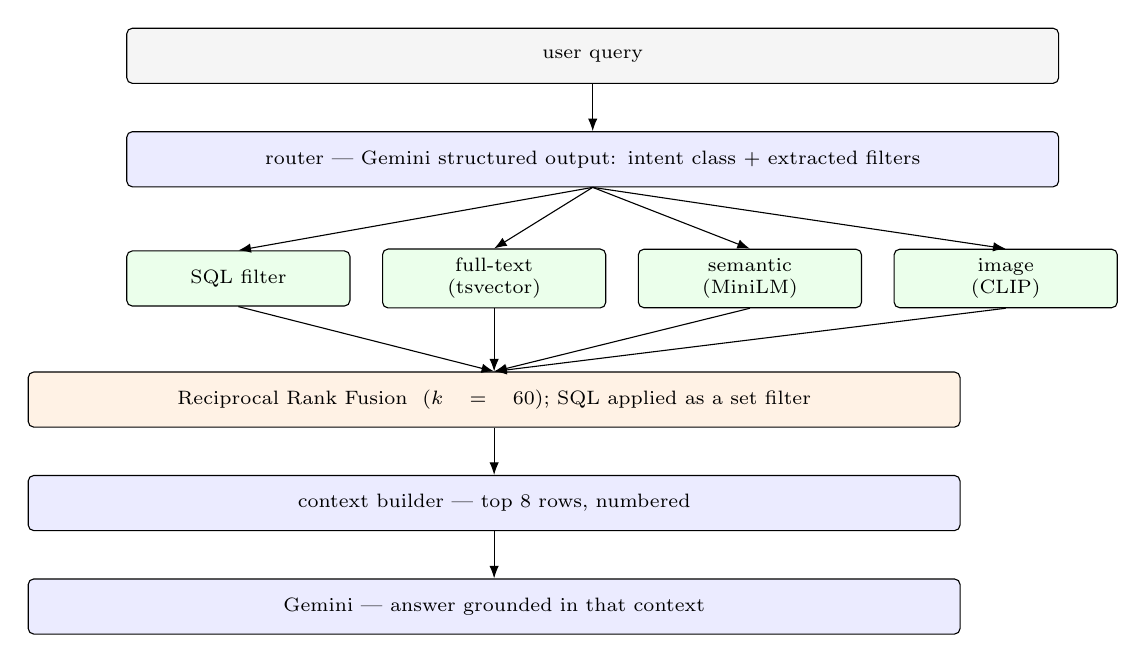
\begin{tikzpicture}[
    node distance=6mm and 4mm,
    stage/.style={draw,rounded corners=2pt,align=center,font=\scriptsize,
                  minimum height=7mm,text width=2.6cm},
    wide/.style={draw,rounded corners=2pt,align=center,font=\scriptsize,
                 minimum height=7mm,text width=11.6cm},
    arr/.style={-{Latex[length=1.6mm]}}
  ]
  \node[wide,fill=gray!8] (q) {user query};
  \node[wide,fill=blue!8,below=of q] (r) {router --- Gemini structured output:
        intent class $+$ extracted filters};

  \node[stage,fill=green!8,below=8mm of r.south west,anchor=north west] (s1) {SQL filter};
  \node[stage,fill=green!8,right=of s1] (s2) {full-text\\(tsvector)};
  \node[stage,fill=green!8,right=of s2] (s3) {semantic\\(MiniLM)};
  \node[stage,fill=green!8,right=of s3] (s4) {image\\(CLIP)};

  \node[wide,fill=orange!10,below=8mm of s2.south] (f)
        {Reciprocal Rank Fusion \ ($k=60$); SQL applied as a set filter};
  \node[wide,fill=blue!8,below=of f] (c) {context builder --- top 8 rows, numbered};
  \node[wide,fill=blue!8,below=of c] (g) {Gemini --- answer grounded in that context};

  \draw[arr] (q) -- (r);
  \draw[arr] (r.south) -- (s1.north);
  \draw[arr] (r.south) -- (s2.north);
  \draw[arr] (r.south) -- (s3.north);
  \draw[arr] (r.south) -- (s4.north);
  \draw[arr] (s1.south) -- (f.north);
  \draw[arr] (s2.south) -- (f.north);
  \draw[arr] (s3.south) -- (f.north);
  \draw[arr] (s4.south) -- (f.north);
  \draw[arr] (f) -- (c);
  \draw[arr] (c) -- (g);
\end{tikzpicture}
\caption{Hybrid retrieval workflow.}
\label{fig:flow}
\end{figure}

The stages are:

\begin{enumerate}[itemsep=2pt]
  \item \textbf{Route.} The query is sent to Gemini with a fixed JSON response
        schema requesting an intent classification and any extractable filters.
        The response is parsed, not pattern-matched.
  \item \textbf{Reconcile filters.} Filters chosen explicitly in the interface
        override anything the router inferred, on the basis that a deliberate
        selection is a stronger signal than the model's reading of a sentence.
  \item \textbf{Retrieve.} The applicable retrievers run and return ranked
        identifier lists. Each over-fetches at twice the requested limit so that
        fusion has sufficient overlap to work with.
  \item \textbf{Constrain.} The structured SQL result is applied as a set
        intersection over those ranked lists --- see
        Section~\ref{sec:filter-not-rank}.
  \item \textbf{Fuse.} Remaining lists are merged with Reciprocal Rank Fusion.
  \item \textbf{Hydrate.} Fused identifiers are resolved back to full rows from
        \texttt{attractions\_full}, with images attached in one batched query.
  \item \textbf{Generate.} The top rows are rendered as numbered context and
        Gemini is prompted to answer using only that context, and to say so when
        the context does not cover the question.
\end{enumerate}

Every response carries the answer, the rows, the context string and the list of
retrievers that ran, so the interface can display the evidence rather than only
the conclusion.

\subsection{Reciprocal Rank Fusion}

The retrievers produce scores that are not comparable
(Table~\ref{tab:scoreranges}). Normalising them onto a shared scale would
require per-retriever calibration that would drift as data was added. RRF
avoids the problem entirely by using only each document's \emph{position} in
each list:

\begin{equation}
\mathrm{score}(d) \;=\; \sum_{i \in R} \frac{1}{k + \mathrm{rank}_i(d)},
\qquad k = 60
\end{equation}

where $R$ is the set of retrievers that returned $d$. The constant $k=60$ is the
value given by Cormack et al.~\cite{rrf}. It damps the gap between the leading
positions, so that a document ranked first by one retriever but absent from the
others does not automatically outrank a document ranked second and third by two
retrievers. Agreement across retrievers is rewarded over dominance within one.

\subsection{Structured retrieval is a filter, not a ranking}
\label{sec:filter-not-rank}

The structured retriever is deliberately \emph{not} one of the lists fed into
fusion. This was not the original design; it was corrected after the defect
described in Section~\ref{sec:defect}.

A SQL result is a \emph{set}. Ours is returned \texttt{ORDER BY name}, which is
an alphabetical ordering, and RRF cannot distinguish that from a relevance
ordering --- it would award whichever attraction sorts first the largest
possible contribution, $1/(60+1)$, purely on account of its initial letter.

Structured retrieval therefore constrains which candidates are \emph{eligible}:

\begin{lstlisting}[language=Python,caption={Structured results applied as an
intersection.}]
allowed_ids = {row["id"] for row in structured_rows}
ranked_lists = {name: [i for i in ids if i in allowed_ids]
                for name, ids in ranked_lists.items()}
\end{lstlisting}

Two details matter. The intersection is applied \emph{after} every retriever has
run, so the constraint also binds the image retriever --- otherwise a beach
could surface under a \texttt{historical\_site} query on visual similarity
alone. And if the intersection is empty the constraint is dropped entirely, so
that a router which misreads a district degrades the ranking rather than
blanking the page.

The general principle: RRF fuses \emph{rankings}. A retriever that does not
produce a genuine relevance ordering belongs in the filter step, not the fusion
step.

\subsection{Lexical query strategy}

Full-text search runs in two passes. \texttt{websearch\_to\_tsquery} requires
every term to be present, which is precise and correct for a query such as
``Sigiriya''. Conversational queries, however, rarely have every term present in
a name or district, so the strict match returns an empty set. When that happens
the terms are re-issued disjunctively via \texttt{to\_tsquery}, surfacing
partial matches and allowing \texttt{ts\_rank} to order them.

% ===========================================================================
\section{Implementation Details}
% ===========================================================================

\subsection{Technology stack}

\begin{table}[h]
\centering
\small
\begin{tabular}{lll}
\toprule
\textbf{Layer} & \textbf{Technology} & \textbf{Rationale} \\
\midrule
Relational store & PostgreSQL 16 (Docker) & Constraints, views, native full-text search \\
Vector store     & ChromaDB               & Local persistence, metadata filtering \\
Text embedding   & \texttt{all-MiniLM-L6-v2} & Fast on CPU, adequate at this corpus size \\
Image embedding  & CLIP ViT-B/32          & Shared image/text vector space \\
Language model   & Google Gemini          & Free tier, structured JSON output \\
Backend          & FastAPI                & Pydantic validation, generated OpenAPI docs \\
Frontend         & HTML, CSS, JavaScript  & No framework, no external assets \\
Language         & Python 3.13            & --- \\
\bottomrule
\end{tabular}
\caption{Technology choices.}
\end{table}

PostgreSQL runs in Docker Compose so that both team members work against an
identical environment. The implementation comprises approximately 2{,}400 lines
of Python across 26 modules and 570 lines of frontend code.

\subsection{API surface}

\begin{table}[h]
\centering
\small
\begin{tabular}{lp{8.4cm}}
\toprule
\textbf{Endpoint} & \textbf{Purpose} \\
\midrule
\texttt{POST /query/structured}    & SQL filters, plus full-text when a keyword is supplied \\
\texttt{POST /query/semantic}      & Dense retrieval over description embeddings \\
\texttt{POST /query/image}         & Text-to-image retrieval via CLIP \\
\texttt{POST /query/image/upload}  & Image-to-image retrieval (multipart) \\
\texttt{POST /query/hybrid}        & Routed, fused, multi-retriever query \\
\texttt{GET /health}               & Database reachability, collection sizes, model configuration \\
\texttt{GET /filters}              & Interface dropdown values, derived from the data \\
\texttt{GET /images/\{...\}}       & Attraction imagery \\
\texttt{GET /ui}                   & The frontend \\
\bottomrule
\end{tabular}
\caption{HTTP endpoints.}
\end{table}

All four query endpoints return an identical response shape, so the interface
requires a single rendering path. Each response includes the \texttt{context}
field --- the exact text passed to the language model --- which the interface
exposes in a collapsible panel so that retrieval can be inspected rather than
taken on trust. A \texttt{generate: false} flag on every request skips the
language-model call, which is the fastest way to time or inspect retrieval in
isolation.

Because the frontend is served by the API at \texttt{/ui}, requests are
same-origin and the entire system runs from a single command.

\subsection{Model selection and quota handling}

Gemini free-tier quotas are enforced per model, and several published model
identifiers report a zero quota or are closed to new API keys --- failures which
superficially resemble an authentication error. The system therefore uses the
\texttt{*-latest} aliases and separates the two workloads:

\begin{itemize}[itemsep=2pt]
  \item \textbf{Routing} uses a lite model. Classification into four labels is
        an easy task, and routing runs on \emph{every} query, so using the
        flagship model here would exhaust the daily allowance before any answers
        were generated.
  \item \textbf{Answer generation} uses the flagship flash model, falling back
        to the lite model on quota exhaustion.
\end{itemize}

\subsection{Graceful degradation}

Two external dependencies can fail. Neither takes the system down.

\begin{table}[h]
\centering
\small
\begin{tabular}{lp{8.6cm}}
\toprule
\textbf{Failure} & \textbf{Behaviour} \\
\midrule
No API key, or quota exhausted & Routing falls back to a keyword heuristic; answers are composed from the retrieved rows and labelled accordingly \\
Text collection empty          & Semantic search returns nothing; SQL and full-text are unaffected \\
Image collection empty         & Image search returns nothing; other modes unaffected \\
Database unreachable           & \texttt{/health} reports \texttt{degraded} and the interface reports it \\
\bottomrule
\end{tabular}
\caption{Degradation behaviour.}
\end{table}

The governing rule is that a failure in the generation layer must never prevent
retrieval from being demonstrated. This is not hypothetical: a rate-limited key
during a live demonstration should reduce answer quality, not produce an error
page.

\subsection{Security considerations}

All filter values reach SQL as bound parameters, never through string
interpolation. This matters more than usual here because some filter values
originate from a language model's output; parameter binding ensures that no
value can alter the structure of the query. Uploads are size-limited and
validated as decodable images before reaching the encoder.

% ===========================================================================
\section{Evaluation}
% ===========================================================================

All measurements below were obtained from the running system against the
40-attraction knowledge base, with language-model generation disabled so that
retrieval output could be observed directly.

\subsection{The retrievers fail on disjoint query types}

This is the central justification for fusing them, so it is demonstrated rather
than asserted. Three queries were issued to full-text and semantic search
independently.

\begin{table}[h]
\centering
\small
\begin{tabular}{p{4.1cm}p{4.3cm}p{5.4cm}}
\toprule
\textbf{Query} & \textbf{Full-text (top 3)} & \textbf{Semantic (top 3)} \\
\midrule
``Yapahuwa'' \newline \emph{exact proper noun}
  & \texttt{yapahuwa}
  & \texttt{yapahuwa}, \texttt{hikkaduwa\_beach}, \texttt{yala\_national\_park} \\
\addlinespace
``wetland birds and flamingos'' \newline \emph{descriptive}
  & \emph{(empty)}
  & \texttt{bundala\_np}, \texttt{kumana\_np}, \texttt{sinharaja} \\
\addlinespace
``Gathering of elephants at a reservoir'' \newline \emph{paraphrase}
  & \emph{(empty)}
  & \texttt{minneriya\_np}, \texttt{udawalawe\_np}, \texttt{kaudulla\_np} \\
\bottomrule
\end{tabular}
\caption{Complementary failure modes.}
\label{tab:complement}
\end{table}

For the proper noun, both retrievers find the target, but note what semantic
search places \emph{behind} it: Hikkaduwa and Yala, two attractions with no
relationship to Yapahuwa beyond surface similarity of the token. Dense
embeddings place rare proper nouns near other rare proper nouns of similar
shape. Lexical matching has no such failure mode.

For the two descriptive queries, full-text returns an \emph{empty set} --- the
terms appear nowhere in any name, location or district, the only fields in the
\texttt{tsvector} --- while semantic search returns the correct answer in first
place both times. Bundala is Sri Lanka's Ramsar-listed wetland and principal
flamingo site; ``the Gathering'' is the specific name for the seasonal elephant
congregation at Minneriya.

Neither retriever dominates. One is strictly better in the first case; the other
is the only one that returns anything at all in the remaining two.

\subsection{A defect: fusing a set as though it were a ranking}
\label{sec:defect}

The most instructive result of the project was a defect rather than a feature.
The hybrid endpoint originally treated structured SQL as a fourth ranked list
and fed it directly into RRF. On the query

\begin{center}\emph{``where can I see leopards on a safari?''}\end{center}

it returned \textbf{Kumana, Kaudulla, Bundala}, whereas plain semantic search on
the same query correctly returned \textbf{Yala} first. The hybrid path was
performing \emph{worse} than one of the retrievers it was assembled from.

The cause was that \texttt{structured\_search} returns rows \texttt{ORDER BY
name}. The router had correctly inferred \texttt{category = national\_park}, so
SQL returned all ten parks in alphabetical order, and RRF cannot distinguish an
alphabetical ordering from a relevance ordering. Bundala sorts first and
therefore collected the largest available reciprocal-rank contribution purely on
account of its initial letter.

\begin{table}[h]
\centering
\small
\begin{tabular}{p{3.6cm}p{5.3cm}p{4.6cm}}
\toprule
\textbf{Query} & \textbf{Before} & \textbf{After} \\
\midrule
leopards on a safari & Kumana, Kaudulla, Bundala & \textbf{Yala}, Kumana, Kaudulla \\
beaches in Galle & Unawatuna, Hikkaduwa, Bentota, \emph{Arugam Bay} & Unawatuna, Hikkaduwa, Bentota \\
UNESCO sites in Matale & Sigiriya, Dambulla, Nalanda, Ritigala, \emph{Hikkaduwa Beach} & Sigiriya, Dambulla \\
\bottomrule
\end{tabular}
\caption{Effect of applying structured results as a filter rather than a ranked
list. Italicised entries are incorrect results eliminated by the fix.}
\end{table}

The stray entries in the ``before'' column are the same defect in a second form:
the image retriever's results were not constrained by the active filters, so a
beach could appear under a historical-site query on visual similarity alone. The
correction --- applying the intersection after all retrievers have run ---
addresses both.

\subsection{Worked fusion example}

\begin{sloppypar}
Query: \emph{``UNESCO ancient sites in Matale worth a day trip''}. The router
returned \texttt{query\_type=hybrid}, \texttt{category=historical\_site},
\texttt{district=Matale} and \texttt{unesco\_only=true}. Semantic, full-text and
image retrieval ran, constrained by the structured filter.
\end{sloppypar}

\begin{align*}
\text{Sigiriya:} &\quad \underbrace{1/(60+1)}_{\text{semantic, rank 1}}
                    + \underbrace{1/(60+1)}_{\text{full-text, rank 1}}
                    = 0.032787\\
\text{Dambulla:} &\quad \underbrace{1/(60+2)}_{\text{semantic, rank 2}}
                    + \underbrace{1/(60+2)}_{\text{full-text, rank 2}}
                    = 0.032258
\end{align*}

Both results are Matale UNESCO sites, which is precisely the correct answer set.
The structured filter reduced the candidate pool to the Matale historical sites,
and within that pool the two retrievers producing genuine rankings agreed on the
order.

\subsection{Router accuracy}

Eight queries, two per intended class, were compared against the keyword
heuristic that serves as the fallback path.

\begin{table}[h]
\centering
\small
\begin{tabular}{p{7.2cm}lcc}
\toprule
\textbf{Query} & \textbf{Expected} & \textbf{Gemini} & \textbf{Heuristic} \\
\midrule
beaches in Galle district                          & structured & \checkmark & $\times$ \\
free historical sites                              & structured & \checkmark & $\times$ \\
somewhere peaceful to watch birds                  & semantic   & \checkmark & \checkmark \\
a place with dramatic cliffs and mist              & semantic   & \checkmark & \checkmark \\
what does Sigiriya look like?                      & image      & \checkmark & \checkmark \\
show me somewhere that looks like a tropical beach & image      & \checkmark & \checkmark \\
which UNESCO sites in Matale are worth a day trip? & hybrid     & \checkmark & \checkmark \\
easy hikes in the hill country with good views     & hybrid     & \checkmark & \checkmark \\
\midrule
\multicolumn{2}{r}{\textbf{Accuracy}} & \textbf{8/8} & \textbf{6/8} \\
\bottomrule
\end{tabular}
\caption{Intent classification accuracy.}
\end{table}

Both approaches agree on the semantic and image classes, which carry strong
surface cues (``looks like'', descriptive phrasing without a proper noun) that a
keyword rule detects as reliably as a model does.

Both failures are the same mistake: the heuristic classifies \emph{pure filter}
queries as hybrid. Its rule is ``names a filter \textbf{and} a category
$\rightarrow$ hybrid'', and ``beaches in Galle district'' satisfies both, so it
cannot separate that query from one which additionally carries a descriptive
element. Distinguishing them requires understanding that ``beaches in Galle'' is
fully answerable by a \texttt{WHERE} clause whereas ``beaches in Galle worth a
day trip'' is not --- which is what the model supplies and a keyword rule
structurally cannot.

The practical cost of the error is modest: a hybrid classification runs
additional retrievers and returns a superset. It is slower and marginally
noisier, not wrong. That is the intended failure mode for a fallback path.

\subsection{Sensitivity to phrasing}

Semantic retrieval is not uniformly robust. Two queries of near-identical intent
produce materially different rankings.

\begin{table}[h]
\centering
\small
\begin{tabular}{lll}
\toprule
\textbf{Query} & \textbf{Top result} & \textbf{Rank of Bundala} \\
\midrule
``wetland birds and flamingos'' & Bundala \checkmark & 1 \\
``a quiet place to watch migrating birds in wetlands'' & Mirissa Beach $\times$ & 4 \\
\bottomrule
\end{tabular}
\caption{Phrasing sensitivity.}
\end{table}

The second phrasing places Mirissa Beach first at similarity 0.3437, ahead of
Kumana (0.3408) and Bundala (0.2826). The probable cause is the words ``quiet''
and ``place to watch'': Mirissa's description is dense with watching language
(whale watching, sunset viewpoint), and the structured prefix folded into every
document contributes a constant component that compresses the score range. All
four leading similarities fall between 0.28 and 0.35 --- a narrow band in which
ranking is fragile.

This is the clearest argument for hybrid retrieval being the default mode:
introducing a second retriever's opinion is what stabilises a ranking this
closely spaced.

\subsection{Observed score ranges}

\begin{table}[h]
\centering
\small
\begin{tabular}{lll}
\toprule
\textbf{Retriever} & \textbf{Metric} & \textbf{Typical range} \\
\midrule
Semantic (MiniLM)        & cosine similarity & 0.28 -- 0.65 \\
Image (CLIP text-to-image) & cosine similarity & 0.15 -- 0.30 \\
Full-text                & \texttt{ts\_rank}  & 0.06 -- 0.99 \\
Structured               & none (set membership) & --- \\
\bottomrule
\end{tabular}
\caption{Score ranges observed during testing.}
\label{tab:scoreranges}
\end{table}

These bands are the concrete reason fusion operates on rank rather than score. A
CLIP similarity of 0.26 represents a strong visual match; a MiniLM similarity of
0.26 is close to noise. Any score-based merge would require per-retriever
calibration and would drift as data was added.

\subsection{Structured retrieval}

Structured retrieval behaves deterministically, as expected of SQL. Filtering on
\texttt{category=beach, district=Galle} returns Bentota, Hikkaduwa and Unawatuna
--- all three correct and complete. Filtering on
\texttt{category=historical\_site, unesco\_only=true} returns exactly the
UNESCO-listed sites.

One design decision is worth recording: \texttt{district} matches with
\texttt{ILIKE '\%...\%'} rather than equality, because several attractions span
two districts (\texttt{Southern/Uva}, \texttt{Ratnapura/Monaragala}). Exact
matching would silently exclude them from any district filter.

\subsection{Limitations}
\label{sec:limitations}

\begin{itemize}[itemsep=3pt]
  \item \textbf{Corpus size.} At 40 attractions, metrics such as precision@$k$
        are not meaningful; with ten items per category, most filtered queries
        can return a large fraction of the category.
  \item \textbf{Image coverage is partial (24 of 40).} Wikimedia rate-limits
        bulk downloads aggressively, and the set was left incomplete rather than
        spending many hours in backoff. Coverage is uneven --- historical sites
        are represented by only three images --- so visual retrieval draws on a
        skewed subset. This bounds image retrieval alone; the other three query
        modes cover all 40 attractions, since they retrieve on text.
  \item \textbf{No ground-truth relevance judgements.} The assessment above is
        qualitative: inspecting results and judging them. A rigorous evaluation
        would require a labelled query set, which is not practical at this
        corpus size.
  \item \textbf{Small router test set.} Eight queries, written by the same
        people who wrote the classifier prompt, is sufficient to show that the
        two paths differ but not to state an accuracy figure with confidence.
  \item \textbf{No numeric price filtering.} \texttt{entrance\_fee} is stored as
        free text (\texttt{"USD 30"}, \texttt{"Free"}, \texttt{"LKR 500
        (foreign) / LKR 50 (local)"}), so a query such as ``under 500 rupees''
        cannot be honoured. The router will classify it as a numeric filter that
        nothing downstream can apply. Only a free-entry predicate exists.
  \item \textbf{Single language.} Both the \texttt{tsvector} configuration and
        the embedding models are English-only.
  \item \textbf{Free-tier quota shapes usage.} The flagship model permits
        roughly twenty requests per day. Routing therefore runs on a lite model,
        and generation degrades to the lite model once the allowance is spent.
\end{itemize}

% ===========================================================================
\section{Conclusion}
% ===========================================================================

The system meets its objective: a single knowledge base of Sri Lankan
attractions, queryable four ways, with generated answers grounded in retrieved
evidence rather than model recall.

Three findings are worth carrying forward. First, lexical and dense retrieval
fail on genuinely disjoint query types --- one returns nothing where the other
succeeds, and vice versa --- which justifies fusion empirically rather than by
assertion. Second, Reciprocal Rank Fusion is a fusion of \emph{rankings}, and
supplying it with a set that carries no relevance order actively degrades
results; the leopard query regression demonstrates this concretely. Third,
structured intent classification by a language model outperformed a keyword
heuristic precisely where the distinction requires understanding rather than
pattern matching, while the heuristic's failure mode proved benign enough to
serve as a fallback.

The most valuable extensions would be broadening image coverage to all 40
attractions, parsing entrance fees into a numeric column to support price
filtering, and assembling a labelled query set so that retrieval quality could
be measured rather than inspected.

% ===========================================================================
\section*{Acknowledgements}
\addcontentsline{toc}{section}{Acknowledgements}
% ===========================================================================

\paragraph{Attraction data.} Compiled from publicly available sources including
Wikipedia and published material from the Sri Lanka Tourism Development
Authority. Coordinates, entrance fees and seasonal information are subject to
change and were current at the time of writing.

\paragraph{Imagery.} All photographs were retrieved from Wikimedia Commons
through the Wikipedia API. Each file retains its own licence, viewable on the
corresponding Commons file page. Per-file attribution --- attraction, source
article and file URL --- is generated automatically by
\texttt{data/fetch\_images.py} and recorded in
\texttt{data/images/IMAGE\_SOURCES.md}, which accompanies the source code
submission.

\paragraph{Models and libraries.}
\begin{sloppypar}
\texttt{sentence-transformers} and \texttt{all-MiniLM-L6-v2} (Reimers and
Gurevych); CLIP ViT-B/32 (OpenAI), accessed through Hugging Face
\texttt{transformers}; Google Gemini; ChromaDB; PostgreSQL; FastAPI; SQLAlchemy;
PyTorch; Pillow.
\end{sloppypar}

\paragraph{AI-assisted tools.}
% ---------------------------------------------------------------------------
% The assignment brief requires an explicit disclosure of AI-assisted tools
% used during development. Edit the sentence below so that it accurately
% describes your own use before submitting. Do not delete the paragraph.
% ---------------------------------------------------------------------------
AI-assisted coding tools were used during development. All design decisions,
schema modelling, evaluation and this report were reviewed and verified by the
authors, and the measurements reported in Section~6 were obtained by executing
the system directly.

% ===========================================================================
\begin{thebibliography}{9}
\addcontentsline{toc}{section}{References}

\bibitem{rrf}
G.~V. Cormack, C.~L.~A. Clarke and S.~B\"uttcher,
\emph{Reciprocal Rank Fusion Outperforms Condorcet and Individual Rank Learning
Methods}, Proceedings of the 32nd International ACM SIGIR Conference on Research
and Development in Information Retrieval, 2009, pp.~758--759.

\bibitem{minilm}
N.~Reimers and I.~Gurevych,
\emph{Sentence-BERT: Sentence Embeddings using Siamese BERT-Networks},
Proceedings of the 2019 Conference on Empirical Methods in Natural Language
Processing, 2019.

\bibitem{clip}
A.~Radford et al.,
\emph{Learning Transferable Visual Models From Natural Language Supervision},
Proceedings of the 38th International Conference on Machine Learning, 2021,
pp.~8748--8763.

\bibitem{pg}
The PostgreSQL Global Development Group,
\emph{PostgreSQL 16 Documentation}, 2024.
\url{https://www.postgresql.org/docs/16/}

\bibitem{chroma}
Chroma, \emph{ChromaDB Documentation}, 2025. \url{https://docs.trychroma.com/}

\end{thebibliography}

\end{document}
